\documentclass[12pt,letterpaper,titlepage]{article}

\usepackage{fontspec}
\defaultfontfeatures{Mapping=tex-text}
\usepackage{xunicode}
\usepackage{xltxtra}
\usepackage{amsmath}
\usepackage{pdfpages}
\usepackage{amsfonts}
\usepackage{bbold}
\usepackage{amssymb}
\setcounter{secnumdepth}{0}
\usepackage{nameref}
\usepackage{enumitem}
\usepackage{environ}
\usepackage{pgfplots}
\usepackage{listings}

\showboxdepth=\maxdimen
\showboxbreadth=\maxdimen


\usepackage{paracol}
\usepackage{wrapfig}
\globalcounter{table}
\globalcounter{figure}
\usepackage{graphicx}
\usepackage[left=1in,right=1in,top=1in,bottom=1in]{geometry}
\graphicspath{{img/}}

\author{Jacob Abel}
\title{	Design \& Simulate 18
	\\\large ECE2204 CRN:82929
}

\setlength{\parskip}{0.5em}

\begin{document}
\maketitle
\begin{raggedright}
\columnratio{0.6}
\begin{paracol}{2}
\switchcolumn
\begin{center}
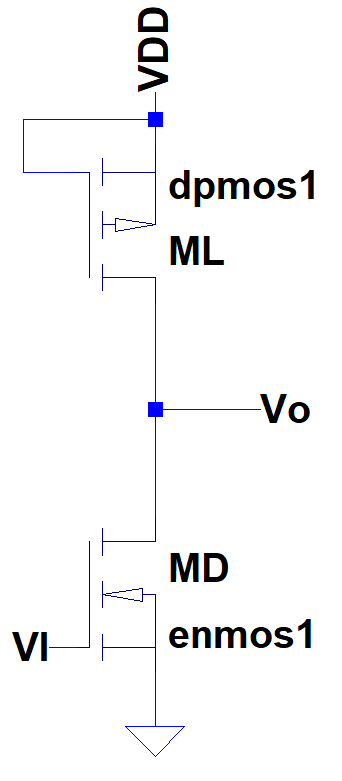
\includegraphics[width=\textwidth, height=15\baselineskip, keepaspectratio=true]{ds1a}
\end{center}
\switchcolumn
\section{Problem 18.3-10.a.1: } 
\subsection{Design}
Determine the modes of the transistors, determine the MOSFETs responsible for each border point, and calculate $V_{in}$ and $V_O$ for each border point. Additionally, determine the power of the circuit for the maximum and minimum $V_{in}$. Assume $V_{TND} = 1V$, $V_{TPL} = 2V$, $K_{ND} = 50\mu A/V^2$, $K_{PL} = 10\mu A/V^2$, and $V_{DD} = 5V$.

\begin{align*}
   V_O
   &= V_{DD} - V_{TPL}
    = 5V - 2V
    = 3V
\\ I_{SL}
   &= K_{PL} V_{SD}^2
    = K_{PL} V_{TPL}^2
    = (10\mu A/V^2)(2V)^2
    = 40\mu A
\\ I_{SL}
   &= K_{ND} (V_I - V_{TND})^2
\\ V_I
   &= \sqrt{\frac{I_{SL}}{K_{ND}}} + V_{TND}
    = \sqrt{\frac{40\mu A}{50\mu A/V^2}} + 1V
    = 1.895V
\\ P_{Vmin}
   &= V_II_{SL}
    = (1.895V)(40\mu A)
    = 75.8\mu W
\end{align*}
\end{paracol}

\begin{align*}
   I_{SL}
   &= K_{PL} (V_{SGL} + V_{TPL})^2
    = K_{PL} (V_{TPL})^2
    = (10\mu A/V^2)(2V)^2
    = 40\mu A
\\ V_O
   &= \sqrt{\frac{I_{SL}}{K_{D}}}
    = \sqrt{\frac{40\mu A}{50\mu A/V^2}}
    = 0.9V
\\ V_I
   &= V_O + V_{TND}
    = 0.9V + 1V
    = 1.9V
\\ P_{Vmax}
   &= V_II_{SL}
    = (1.9V)(40\mu A)
    = 76\mu W
\end{align*}

Initially, the circuit is in region 1 and therefore $ML$ is in the Ohmic Mode and $MD$ is off. Between $V_I = 1.895$ and $V_I = 1.9V$ the circuit is in region 2 and both transistors switch to Saturation Mode. Past $V_I = 1.9V$, the circuit enters region 3 and $ML$ transitions back into Ohmic Mode.

At the first transition $V_O = 3V$ and $P_{Vmax} = 76/mu W$. At the second transition  $V_O = 0.9V$ and $P_{Vmin} = 75.8/mu W$.

\clearpage
\subsection{Validation}

\begin{center}
LTSpice Implementation
\columnratio{0.32}
\begin{paracol}{2}
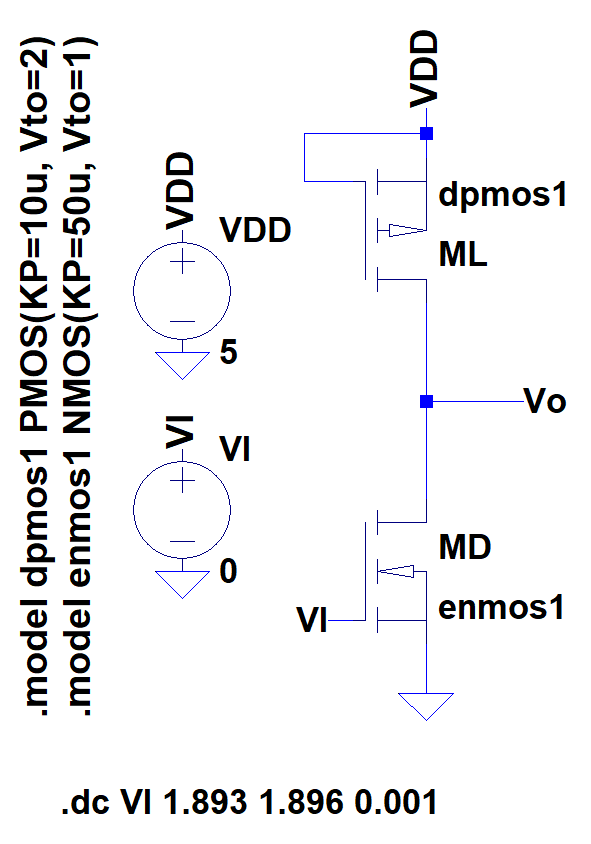
\includegraphics[width=.31\textwidth, height=\textheight, keepaspectratio=true]{ds1b}
\switchcolumn
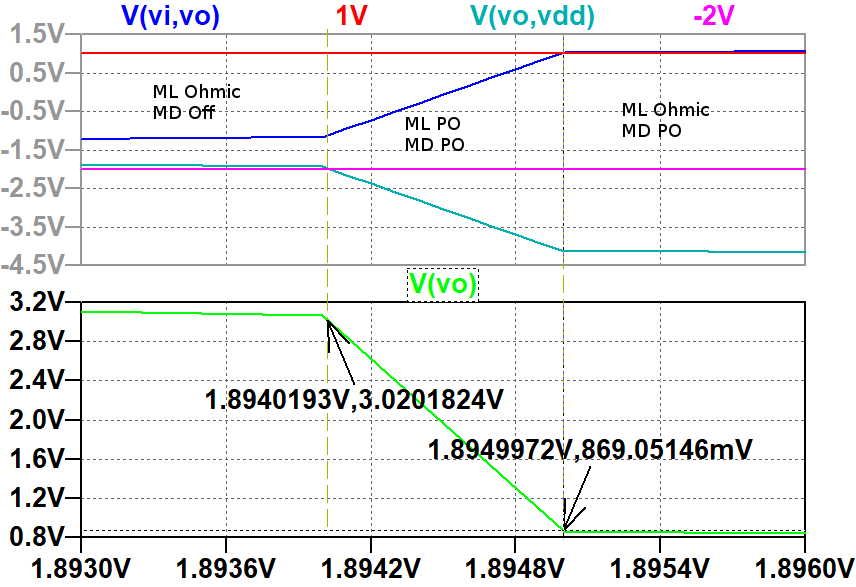
\includegraphics[width=.62\textwidth, height=\textheight, keepaspectratio=true]{ds1c}
\end{paracol}
\begin{align*}
   Err_{V_{I1}} &= \frac{|1.895 - 1.894|}{1.895} = 0.05\%
\\ Err_{V_{I2}} &= \frac{|1.9 - 1.895|}{1.9} = 0.26\%
\\ Err_{V_{O1}} &= \frac{|3 - 3.02|}{3} = 0.60\%
\\ Err_{V_{O2}} &= \frac{|0.9 - 0.869|}{0.9} = 3.4\%
\end{align*}

Deviation on $V_{O2}$ is due to marker placement error.

\end{center}


This assignment should demonstrate a basic ability to manipulate, design, and analyse depletion load MOSFET circuits.

\textit{I have neither given nor received unauthorized assistance on this assignment.}


\end{raggedright}
\end{document}
